\documentclass[twocolumn,showpacs,preprintnumbers,nofootinbib,prd,
superscriptaddress,10pt]{revtex4-2}

\usepackage{amsmath,amssymb}
\usepackage{amsfonts}
\usepackage{mathtools}
\usepackage[normalem]{ulem}
\usepackage{textcomp}
\usepackage{enumitem}
\usepackage{bm}
\usepackage{bbm}
\usepackage{afterpage}
%\usepackage{float}
\usepackage{graphicx}
\usepackage{subcaption}
\graphicspath{{img/}} %setting img path

\usepackage{tabularx, longtable, makecell}
\usepackage{multirow}
\usepackage{arydshln}

\usepackage{tensor}
\usepackage{layouts}
\usepackage[usenames,dvipsnames]{xcolor}
\usepackage[utf8]{inputenc}
\usepackage{algorithm}
\usepackage{algpseudocode}
\usepackage{rotating}
\usepackage{hyperref}
%\usepackage{ragged2e}
\usepackage{blindtext}
\usepackage{graphicx}
\usepackage{siunitx}
	\sisetup{output-decimal-marker={.}}
	
	%some math symbols
\newcommand{\R}{\mathbb{R}}
\newcommand{\N}{\mathbb{N}}
\DeclareMathOperator{\sign}{sign}
\renewcommand{\d}[1]{\ensuremath{\operatorname{d}\!{#1}}}
\newcommand{\dvol}[2]{\ensuremath{\operatorname{d}^{#2}\!{#1}}}
%argmin and argmax
\DeclareMathOperator*{\argmax}{arg\,max}
\DeclareMathOperator*{\argmin}{arg\,min}

\newcommand{\scalar}[2]{\langle #1|#2 \rangle}
\newcommand{\scalarnonorm}[2]{\langle #1|#2 \rangle_{\text{not normalized}}}
\newcommand{\rescalar}[2]{( #1|#2 )}
\newcommand{\imscalar}[2]{[ #1|#2 ]}


% comments command
\newcommand{\stefano}[1]{{\textcolor{blue}{\texttt{SS: #1}} }}
\newcommand{\sarah}[1]{{\textcolor{red}{\texttt{SC: #1}} }}
\newcommand{\bhooshan}[1]{{\textcolor{cyan}{\texttt{BG: #1}} }}
\newcommand{\oldnewtxt}[2]{\sout{#1}\textcolor{red}{#2}}


\begin{document}

	%%%%%%%%%%%%%%%%%%%%%%%%%%%%%%%%% ABSTRACT
\begin{abstract}
	We introduce a novel method to generate a bank of gravitational-waveform templates of binary black hole (BBH) coalescences for matched-filter searches in LIGO, Virgo and Kagra data. Unlike the standard approach, our method relies on a numerical metric approximation of the distance between templates, which makes the template placement orders of magnitude faster than with existing techniques.
	Our method applies to a variety of different manifolds of signals and is particularly suitable for covering high dimensional spaces, such as those associated with precessing and/or eccentric waveforms.
	We compare our method with the state-of-the-art stochastic placement code and we find that our code slightly overcovers the space, while achieving similar efficiency in recovering signals. To demonstrate the capabilities of our code, we generate a precessing bank, an intermediate mass black hole bank with higher-order modes, and an eccentric bank, and show that they cover the space in a satisfactory way.
	Our publicly released code \texttt{mbank} will enable searches of high dimensional regions of BBH signal space, hitherto unfeasible due to the prohibitive cost of bank generation.
\end{abstract}
	
	%%%%%%%%%%%%%%%%%%%%%%%%%%%%%%%%% TITLE
	\title{Metric template placement for high dimensional regions of compact binary mergers}
	\author{Stefano \surname{Schmidt}}
		\email{s.schmidt@uu.nl}
        \affiliation{Nikhef, Science Park 105, 1098 XG, Amsterdam, The Netherlands}
        \affiliation{Institute for Gravitational and Subatomic Physics (GRASP),
Utrecht University, Princetonplein 1, 3584 CC Utrecht, The Netherlands}

	\author{Bhooshan \surname{Gadre}}
        \affiliation{Institute for Gravitational and Subatomic Physics (GRASP),
Utrecht University, Princetonplein 1, 3584 CC Utrecht, The Netherlands}
        
        %
	\author{Sarah \surname{Caudill}}
%        \affiliation{Nikhef, Science Park 105, 1098 XG, Amsterdam, The Netherlands}
%        \affiliation{Institute for Gravitational and Subatomic Physics (GRASP),
%Utrecht University, Princetonplein 1, 3584 CC Utrecht, The Netherlands}
		\affiliation{Department of Physics, University of Massachusetts, Dartmouth, MA 02747, USA}
		\affiliation{Center for Scientific Computing and Visualization Research, University of Massachusetts, Dartmouth, MA 02747, USA}
	\maketitle

	%\tableofcontents

	%%%%%%%%%%%%%%%%%%%%%%%%%%%%%%%%% BODY 
\section{Introduction}

As gravitational waves (GWs) astronomy enters in a mature state, the parameter space of Binary Black Holes (BBH) being searched in the interferometer data by LIGO \cite{LIGOScientific:2014pky} and Virgo \cite{VIRGO:2014yos} Collaborations is constantly increasing. Besides standard searches of BBH \cite{GWTC-1,GWTC-2,GWTC-2.1, GWTC-3}, there have been already searches targeting the parameter space of sub-solar mass black holes (BH) \cite{SSM_O2, SSM_O3a, PhysRevD.106.023024}, primordial BHs \cite{PBH}, eccentric binaries \cite{PhysRevD.102.043005, PhysRevD.104.104016, Nitz:2019spj} and intermediate mass BHs (IMBH) \cite{IMBH_O2, IMBH_O3, Chandra:2022ixv}. Moreover, there is a growing interest in searches for precessing signals \cite{PhysRevD.89.024010, PhysRevD.97.023004, PhysRevD.102.041302, Indik:2016qky}.
All these searches need accurate template banks that covers the parameter space of interest. A template bank gathers a set of GW signals that will be searched in the data with matched filtering \cite{Owen:1998dk}. Their generation can be computationally expensive task and it is crucial for the outcome of state-of-the-art searches.

The most widely used approach to bank generation - the {\it stochastic} method \cite{PhysRevD.80.104014, sbank} - consists in scattering templates around the parameter space with a rejection technique \cite{DalCanton:2017ala, Mukherjee:2018yra, Indik:2016qky, Lenon:2021zac}. A proposed template is included in the bank only if its ``distance" (more precisely mismatch) with all the proposed templates in the bank is larger than the user defined threshold.
While this method is proven to work in many cases, it is computationally demanding, since it requires to generate a huge number of BBH waveforms template and to perform expensive match computations.
With the ever growing parameter space hyper-volume for BBH searches in the strive to more accurate searches, current approaches may become computationally unfeasible.

Revitalizing a pioneering line of research in bank generation \cite{owen_metric, Messenger:2008ta}, there has been recently an increasing attention on {\it metric template placement} \cite{Roy:2017oul, 2018cosp...42E2899R, Coogan:2022qxs, Hanna:2022zpk}, aiming to speed up the template placement.
Such methods rely on approximating the distance (or match) between two waveforms with a bilinear form. Despite being approximate, is allows for a faster template placing that may overcome some of the major limitations of the standard stochastic placement algorithm.

In this work, we develop a novel approach to template placing based on the metric approximation of the mismatch.
Our method is specifically designed for dealing with high-dimensional (more than 4 dimensional) template banks of GWs signals, making it particularly suitable to generate template banks for precessing and eccentric signals.

%Our model constructs an internal representation of the parameter space of interests, computes the metric for distance computation and exploits this for fast template placing.
The approach is implemented in an open-source, production-ready, python package \texttt{mbank}, available on GitHub\footnote{
It is available at the repository \href{https://github.com/stefanoschmidt1995/mbank}{stefanoschmidt1995/mbank}.}
and on the PyPI repository\footnote{
In the PyPI repository, the package is distributed under the name \texttt{\href{https://pypi.org/project/gw-mbank/}{gw-mbank}}.
}.
The package offers support for tiling the parameter space of interests and placing templates with an user defined minimal match. Moreover, it offers an injection helper that allows for a very fast validation of the bank.
As a summary, \texttt{mbank} is implemented to be:
\begin{itemize}
	\item Orders of magnitude faster than the state-of-the-art
	\item Suitable to cover a high dimensional parameter space
	\item Close to provide optimal coverage
\end{itemize}

The rest of this paper is devoted to present and describe \texttt{mbank}.
In Sec.~\ref{sec:methods} we present the details of the bank generation algorithm.
Sec.~\ref{sec:validation} will be devoted to the validation of the performance of the code. We assess the accuracy of the metric approximation and of the template placing methods we implemented. We also compare our method with the widely used stochastic placement code \texttt{sbank} \cite{sbank}.
To demonstrate the capabilities of \texttt{mbank}, in Sec.~\ref{sec:bank_generation}, we present three large banks covering ``exotic" regions of parameter space: a bank of precessing signals, a bank of Intermediate Mass Black Hole (IMBH) with Higher Order Modes (HM) and a bank of eccentric signals.
Finally, in Sec.~\ref{sec:conclusion} we will present some conclusive remarks, with particular attention to future prospects.

	%%%%%%%%%%%%%%%%%%%%%%%%%%%%%%%%%
\section{Methods} \label{sec:methods}

When searching for a BBH signal in GW data, it is custom to use a frequentist detection statistics $\Lambda$ \cite{Creighton_book, PhysRevD.94.024012}.
We model the detector output $s(t)$ to be composed of {\it Gaussian} noise $n(t)$ and possibly by a known GW signal $h(t)$.
Given some observed data $d(t)$, the detection statistics is then a measure of the (log)probability ratio between the signal hypothesis $s = n+h$ and the noise hypothesis $s = n$.
In symbols:
\begin{equation}\label{eq:LL}
	\Lambda(\theta) = \log\frac{p(s = n+h(\theta)|d)}{p(s = n|d)}
\end{equation}
where a signal model is parameterized by a vector of parameters $\theta$, which represents a GW signal $h(t;\theta)$.
For any given observation time, a search aims to maximize the detection statistics with respect to $\theta$. 

The generic eccentric BBH signal registered at detector is characterized by 17 quantities \cite{Sathyaprakash_2009}, grouped into \textit{intrinsic} and \textit{extrinsic} parameters.
The twelve intrinsic parameters are needed to fully characterize the source: they consist in two BH masses ($m_1$, $m_2$), two 3 dimensional spins ($\mathbf{s}_1$, $\mathbf{s}_2$), the inclination angle $\iota$, the reference phase $\phi$, the eccentricity $e$ of the orbit and the mean periastron anomaly $a$.
Five extrinsic parameters characterizes the position of the source with respect to the observer: they are sky location (two angles: right ascension and declination), luminosity distance $D$, polarization angle $\Psi$ and the time of arrival of the signal.

It turns out that one is able to maximize analytically $\Lambda(\theta)$ over the extrinsic parameters and, depending on the scope of the search, over many of the intrinsic parameters\footnote{
In the case of a a non-precessing BBH, where we neglect the Higher Order Modes (HM) of the waveforms, the parameters space to search by brute force has only 4 dimensions (the two masses and the two z components of the spins).
}.
For the other quantities, a brute force approach is required, where $\Lambda(\theta)$ is evaluated on a large set of values of $\theta$, called {\it template bank} \cite{PhysRevD.77.104017, Mukherjee_2021}.
A GW search filters the data with the templates of a bank and computes the detection statistics for each template as a function of time: this technique, called {\it matched filtering}, is implemented by several pipelines to successfully search for GW signals \cite{Usman:2015kfa,PhysRevD.95.042001,gstlal_paper2, Aubin:2020goo, Chu:2020pjv}.

It is useful, to think of the BBH parameter space as a D-dimensional manifold $\mathcal{B}_D$, embedded in a large 12 dimensional manifold $\mathcal{B}$: each point of the manifold corresponds to a GW signal. The number $D$ of dimensions depends on the BBH variables under consideration.
As the parameters that do not enter the interesting space can be freely neglected (i.e. set to $0$ or to a meaningful default value), the manifold $\mathcal{B}_D$ is effectively a lower dimensional {\it projection} of the full manifold $\mathcal{B}$.

%Placing templates on $\mathcal{B}_D$ is a highly non-trivial task, as one has to struggle to ensure a good coverage (and avoid missing any signal) while keeping a low number of templates (and save computational power).
%Throughtout the years many different techniques have been devised to achieve such goal.
%
To place templates on $\mathcal{B}_D$, it is standard to equip the manifold with a distance (called {\it mis-match}) and then place templates so that: (i) they cover all the manifold and (ii) their mutual distance is as close as possible to a target distance.
Building on this, we develop a novel approach to template placing in three steps:

\begin{enumerate}
	\item Construction of a metric approximation of the match between templates. This makes $\mathcal{B}_D$ a Riemannian manifold.
	\item Creation of a tiling (cover) for the manifold. In each tile the metric is assumed to be constant.
	\item Placing the templates according to the tiling
\end{enumerate}

Although the template placing is only approximately optimal, our method is order of magnitude faster than the standard approach, as it avoids to compute a large number of waveforms.
We will devote the rest of this section to go through all the details of the steps above.

\subsection{The metric} \label{sec:metric}

In this section we define a metric distance on the manifold of templates $\mathcal{B}_D$. Such metric approximates the {\it mis-match} between templates and can be used a fast-to-compute surrogate. We will also derive an explicit expression for the metric in terms of the waveform and its gradients.

Under the assumption of Gaussian noise \cite{Creighton_book}, it is natural to introduce a complex \textit{scalar product}\footnote{
Technically, this is a scalar product on the $L^2$ space of the waveforms $h$.
Moreover, the search likelihood Eq.~\eqref{eq:LL} will depend only $\scalar{h}{h}$ and $\scalar{s}{h}$.
} between two \textit{waveforms} $h$ as:

\begin{equation} \label{eq:scalar_product}
	\scalar{h(\theta_1)}{h(\theta_2)} = 4 \int_{0}^{\infty} \d{f} \frac{\tilde{h}^*(f;\theta_1) \tilde{h}(f;\theta_2)}{S_n(f)}
\end{equation}

where $\tilde{h}(\cdot; \theta)$ denotes the frequency waveform evaluated at the point $\theta$ of the manifold.
For non-precessing circular BBHs, $h(f; \theta) = A(f; \theta) e^{i\phi(f; \theta)} = h_+ + i h_\times$. This however is not valid in the more general case of a precessing and/or eccentric binary. In this case, the form of the likehood changes \cite{Harry:2016ijz, PhysRevD.97.023004, PhysRevD.94.024012}, depending on physical assumptions about the signal, yielding in principle to a different form for the scalar product. Here, however, we neglect this fact and we consider only the physical content of the plus polarization\footnote{
We note incidentally that our assumption is equivalent to considering only signals coming at the interferometer with a zero right ascension and polarization angle.}:
$h = A(f,\theta) e^{i\phi(\theta)} = h_+$. We defer to future studies the discussion of a more general scalar product.

%It is important to note that the parameters $\theta$ may not fully specify the BBH parameter space: in this case, the expression $h(\theta)$ assumes that the waveform is generated at some default constant paramters for the quantities not constrained by $\theta$. Eq.~\eqref{eq:scalar_product} is a measure of the detection statistics $\Lambda(\theta_1)$ that is measured when a signal $h(t; \theta_2)$ is present in the data.

A waveform $h(\theta)$ can be normalized using the scalar product above:
\begin{equation} \label{eq:normalization}
	\hat{h}(\theta) = \frac{h(\theta)}{\scalar{h(\theta)}{h(\theta)}}.
\end{equation}

%We can use the scalar product to define the sought for distance between signals.
For each parameter $t$, we define the overlap $\mathcal{O}(\theta_1,\theta_2, t)$ between normalized WFs as:
\begin{align}\label{eq:overlap}
	\mathcal{O}(\theta_1,\theta_2, t) &= \left\lvert \int\limits_{0}^{+\infty} \d{f} \frac{\tilde{\hat{h}}^*(f;\theta_1)\tilde{\hat{h}}(f;\theta_2) e^{i2\pi ft}}{S_n(f)} \right\rvert \nonumber\\
	&= \lvert \scalar{\hat{h}(\theta_1)}{\hat{h}(\theta_2)e^{i 2\pi ft}} \rvert
\end{align}
where we defined $\hat{h}(\theta)e^{i 2\pi ft}$ to be the waveform $\hat{h}(\theta)$ translated by a constant time $t$ and $\lvert \cdot \rvert$ denotes the absolute value of a complex number.

Based on the overlap, we can eventually define the {\it match} as:
\begin{equation}\label{eq:match}
	\mathcal{M}&(\theta_1,\theta_2) = \max_t \mathcal{O}(\theta_1,\theta_2, t) \\
	%&= \max_t \sqrt{ \rescalar{\hat{h}(\theta_1)}{\hat{h}(\theta_2)e^{i 2\pi ft}}^2 + \imscalar{\hat{h}(\theta_1)}{\hat{h}(\theta_2)e^{i2\pi ft}}^2 }  \nonumber 
\end{equation}
%
The match takes values in the range $[0,1]$ and trivially $\mathcal{M}(\theta,\theta) = 1$.
It amounts to the scalar product between $h(\theta_1)$ and $h(\theta_2)$, maximized over a constant time shift between the two.

We are now ready to define a {\it distance} $d(\theta_1,\theta_2)$ \footnote{
From a strict geometrical point of view, this is not a distance since it does not satisfy triangular inequality. However, this does not affect its effectiveness in measuring the ``dissimilarity" between two waveforms and it will be used regardless.}
on the D-manifold $\mathcal{B}_D$:
\begin{align}\label{eq:distance}
	d(\theta_1,\theta_2) \vcentcolon= \sqrt{1 - \mathcal{M}(\theta_1,\theta_2)}
\end{align}
The quantity $1-\mathcal{M}$ above is also called {\it mismatch}.

To construct the metric approximation of the distance, we replace the distance with a bilinear form in the neighborhood of any point $\theta$. Such bilinear form is represented by a $D\times D$ matrix $M(\theta)$ such that\footnote{
In this expression and everywhere else, we assume Einstein summation convention for vector product.}:
\begin{align}\label{eq:metric_definition}
	d^2(\theta_1,\theta_2) = 1 - \mathcal{M}(\theta_1,\theta_2) \simeq M_{ij}(\theta) \Delta\theta_i \Delta\theta_j
\end{align}
where $\Delta\theta = \theta_1-\theta_2$ is a D-dimensional vector.
The distance induced by the metric approximates the distance between two points of the manifold.
It is worth noting that, like any expansion, Eq.~\eqref{eq:metric_definition} is guaranteed to be accurate only in the limit of small $||\Delta\theta||$\footnote{Here $||\cdot||$ is the usual Euclidean $L^2$ norm.}.
%For $||\Delta\theta|| \gtrsim 1$ the metric approximation may lose its predictivity power and the validity of the approximation needs to be checked in every situation.

Of course, there is not a ``true" expression for the matrix $M_{ij}(\theta)$, but its value may depend on the application and on the range of applicability of the approximation.
A fair guess for the tensor field $M_{ij}(\theta)$ can be done through an optimization problem where we try to minimize the discrepancy between the metric distance Eq.~\eqref{eq:metric_definition} and the actual distance Eq.~\eqref{eq:distance}.
The disagreement of the two distances around a point $\theta$ can be encoded into a {\it loss function}, which depends on the values of the matrix elements $M^\prime_{ij}$:
\begin{equation} \label{eq:loss_function}
	\mathcal{L}_\theta(M^\prime_{ij}) &= \hspace{-4em} \int\limits_{\hspace{3em}\{d(\theta,\theta^\prime) < d_{target}\}} \hspace{-3.8em}
		\dvol{\theta^\prime}{D}  \left[ d^2(\theta,\theta^\prime) - M^\prime_{ij} \Delta\theta_i \Delta\theta_j \right]^2
\end{equation}
where the integration extends on a D-ball with radius $d_{target}$ centered around theta.
The value $d_{target}$ is a tunable parameters which controls the range of validity of the approximation.

At a given point $\theta$, the components $M_{ij}(\theta)$ of the metric are selected by minimizing the above loss:
\begin{equation} \label{eq:metric_optmization}
	M_{ij}(\theta) = \argmin_{M^\prime_{ij}}  \mathcal{L}_\theta(M^\prime_{ij})
\end{equation}
Although the problem can be tackled using standard optimization techniques, in most cases it is unfeasible to do so\footnote{
Future work may try to tackle this optimization problem finding a solution at a feasible computational cost.},
since it requires to evaluate many times $d(\theta,\theta^\prime)$ Eq.~\eqref{eq:distance} and to sample from a ``complex" set such as $\{d(\theta,\theta^\prime) < d_{target}\}$.

To make the metric generation feasible, we find a faster {\it heuristic} solution to Eq.~\eqref{eq:metric_optmization} by identifying the metric $M_{ij}(\theta)$ with the bilinear term of the Taylor expansion of the match.
It depends on the gradients $\partial_i h(\theta)$ of the waveform and has the following expression \cite{owen_metric}:
\begin{equation}\label{eq:metric_expression}
	M_{ij}(\theta) = - \frac{1}{2} \left( H_{ij} - \frac{H_{ti}H_{tj}}{H_{tt}} \right)
\end{equation}
where $H(\theta)$ is the Hessian of the overlap Eq.~\eqref{eq:overlap}, a $D+1$ square matrix.
Note that the metric is positive definite. The details of the computation of the Hessian in terms of the gradients of the waveform are presented in appendix \ref{app:metric}. The full expression is given in Eqs.~\eqref{eq:H_tt_grad}-\eqref{eq:H_ij_grad}.

For most of the waveform models available, the gradients can be evaluated with finite difference methods. For a limited number of Machine Learning based models \cite{Khan:2020fso, PhysRevD.103.043020, ML_wf_model, Tissino:2022thn}, such gradients are available analytically.

%%%
%%%%%%%%% THIS PART IS ABOUT THE PARABOLIC FIT HESSIAN: AS IT DOES NOT REALLY WORK. IT IS PROBLEMATIC TO MENTION IT IN THE PAPER.
%Despite being the most common approach, the hessian metric approximation tends to {\it undestimate} the small eigenvalues of the metric $M$. Whenever this happens, the metric loses its predictivity (especially at large coordinate distances $||\Delta\theta||$), as it will be shown in fig.~\ref{fig:metric_accuracy_distance}. The reason for that is that the gradients are computed with a small finite difference step $\epsilon \sim 10^{-5}$, while the metric is used to make predictions at larger values $\epsilon \sim 1$. A possible solution to this problem is to update the eigenvalues of the Hessian Eq.~\eqref{eq:metric_expression} with those computed by looking at the match at larger distances. For each eigen-direction $\hat{\lambda}_i$, we place a number of points along $\hat{\lambda}_i$ at difference distances $\epsilon$ and we compute the mis-match with the center $\theta$. The i-th eigenvalue $\lambda_i$ is then computed by a parabolic fit of the relation mismatch-distance. In general, the metric with the newly calibrated eigenvalues tends to have much larger eigenvalues but provides a more accuracte representation of the local behavior of the match. We call this metric {\it parabolic fit hessian}. Which version of the metric - {\it hessian} or {\it parabolic fit hessian} - to use is a matter of applications.

Equipped with the metric Eq.~\eqref{eq:metric_expression}, the manifold $\mathcal{B}_D$ becomes a Riemannian manifold with line element:
\begin{equation}\label{eq:line_element}
	\d{s^2} = M_{ij}(\theta) \d{\theta_i} \d{\theta_j}
\end{equation}
We can then use standard results from differential geometry to compute distances and volumes. In particular, the volume of a subset $\mathcal{T}$ (tile) of the manifold can be computed as:
\begin{equation}\label{eq:volume_tile}
	\text{Vol}(\mathcal{T}) = \int_\mathcal{T} \dvol{\theta}{D} \; \sqrt{|M(\theta)|}
\end{equation}
where $|\cdot|$ denotes the determinant of a matrix.

%As a final remark, we note that other definitions for the match are possible (see e.g. \cite{PhysRevD.94.024012,PhysRevD.97.023004}). These are motivated by different expressions for the detection statistics, which depends on the assumptions made on the signal (i.e. precessing or eccentric signals or with Higher Order Modes). Here we limit to use the ``vanilla" expression~\eqref{eq:match} for aligned spins BBH (for which $\tilde{h}_+ \propto i \tilde{h}_\times$), even for cases where it does not hold. We expect the error introduced by this to be negligible.

\subsection{The tiling} \label{sec:tiling}

The metric $M_{ij}(\theta)$ is a continuous quantity, defined at every point $\theta$ of the manifold $\mathcal{B}_D$.
However, it is unfeasible to evaluate the metric whenever a (mis)match computation is required.
To speed up the metric computation on $\mathcal{B}_D$, the parameter space of interest should be divided into different {\it tiles} (subsets), where we assume that the metric can be approximated as a constant within each tile.
%The validity of this assumption will be assesed in Sec.~\ref{sec:tiling_accuracy}.

To simplify the geometry and make the computation faster, we only consider hyper-rectangles as tiles. A tile $\mathcal{T}$ is an ordered couple:
\begin{equation} \label{eq:tile}
	\mathcal{T} = \left(R_{[\theta_{min}, \theta_{max}]}, M \right)
\end{equation}
where $R_{[\theta_{min}, \theta_{max}]}$ is an hyper-rectangles with extrema $\theta_{\text{min/max}}$ and where $M$ is the metric evaluated Eq.~\eqref{eq:metric_expression} at the center of the tile $\frac{\theta_{min}+\theta_{max}}{2}$.

Similarly to \cite{Hanna:2022zpk}, we use the function \texttt{SplitTile} to split a tile $\mathcal{T}$ in 3 tiles $\mathcal{T}_{left}$, $\mathcal{T}_{center}$, $\mathcal{T}_{right}$.
The three resulting tiles are further split if the metric determinants $|M_{right}|, |M_{left}|$ of the left and right tile satisfy:
\begin{equation}
	0.5\left|\log_{\textrm{10}}\frac{|M_{right}|}{|M_{left}|}\right| > \epsilon,
\end{equation}
where the threshold $\epsilon$ can be freely chosen by the user and controls the total number of tiles being generated.
This condition makes sure that the volume element $\sqrt{|M(\theta)|}$ does not change too much between neighboring tiles.
Function \texttt{SplitTile} is described in Alg.~\ref{alg:tiling}.

The tiling generation algorithm iteratively splits an initial tile $\mathcal{T}_{0}$ which covers the space of interest, until all the tiles satisfy the condition above.
To prevent the algorithm from running indefinitely, we may also impose an (optional) threshold \texttt{max-depth} on the number of ``generations of tiles". If set, this limits the number of tiles to $3^{\texttt{max-depth}}$.

As we limit to rectangular tiles, \texttt{mbank} is not able to deal with a non rectangular boundaries for the parameter space. This is of course a strict limitation, as the typical user may want to impose non cubic boundaries. However, due to the speed of the bank generation, a feasible approach to overcome this is to generate the bank on a larger domain and imposing any non-linear boundary as a post processing step. 

The tiling defines a {\it fast} approximation $M^{\text{tiling}}_{ij}(\theta)$ to the true metric $M_{ij}(\theta)$ Eq.~\eqref{eq:distance}:
\begin{equation}\label{eq:metric_tiling}
	M^{\text{tiling}}_{ij}(\theta) = \sum_{k} \mathbf{1}_{R_k}(\theta) M^{k}_{ij}
\end{equation}
where $\mathbf{1}_{R_k}(\theta)$ is the indicator function on the rectangle $R_k$ of the k-th tile and the sum runs over all the tiles $\mathcal{T}_k$ of the tiling. The matrix $M^{k}_{ij}$ is the metric evaluated at the center of the rectangle $R_k$ as in Eq.~\eqref{eq:tile}.


It is important to realize that a tiling defines also an approximation $p^{\text{tiling}}$ to the uniform probability distribution $p(\theta) \propto \sqrt{|M(\theta)|}$\footnote{
A probability distribution is said to be {\it uniform} if, for every volume $V$ of the space, it satisfies $p(V) \propto \text{Vol}(V)$.}
on $\mathcal{B}_D$:
\begin{equation}\label{eq:tiling_pdf}
	p^{\text{tiling}}(\theta) \propto \sum_{\mathcal{T}_k} \mathbf{1}_{R_k}(\theta) \sqrt{|M_k|}
\end{equation}
The equation above can be used to uniformly draw random templates on the space and it will be used widely for template placing.

	%the [H] option is mandatory for revtex4-2: otherwise it throws errors
\begin{algorithm}[H]
	\centering
	\caption{Tiling splitting function}\label{alg:tiling}
	\flushleft
	\hspace*{\algorithmicindent} \textbf{Input}: A tile $\mathcal{T} = \left(R, M\right)$ \\
	\hspace*{\algorithmicindent} \textbf{Output}: Three new tiles
	\begin{algorithmic}
		\Procedure{SplitTile}{$\mathcal{T}$}
		\State $d \gets $ smaller (metric) dimension of $R$
		\State $R_{left}, R_{center}, R_{right} \gets $ 3 equal volume rectangles generated splitting $R$ along dimension $d$ 
		\State $M_{left}, M_{center}, M_{right} \gets $ metric evaluated at the center of each rectangle
		\State\Return{$\mathcal{T}_{left}$, $\mathcal{T}_{center}$, $\mathcal{T}_{right}$}
		\EndProcedure
	\end{algorithmic}
\end{algorithm}


\subsection{Template placing} \label{sec:template_placing}

Once a tiling is available, we need to place the templates that will be part of the bank.
As it is common, the input parameter controlling the average spacing of the templates and their number is the so-called {\it minimum match} $MM$. It is defined as the minimum tolerable match that a random injection (inside the relevant space) must have with the templates of the bank.

A variety of template placing methods have been implemented in \texttt{mbank}, each of which has their own strength and applicability.
Below, we describe briefly the most interesting among them and in Sec.~\ref{sec:placing_accuracy}, we make quantitative studies on their performance\footnote{
This list is not exhaustive: more placing methods are implemented and documented, although not fully validated, in \texttt{mbank}.}.

\paragraph{Uniform}\label{par:uniform}
The templates are randomly drawn from the probability distribution defined by the metric $p(\theta) \propto \sqrt{M(\theta)}$, as described in \cite{Messenger:2008ta}.
Of course, we only have access to the approximation Eq.~\eqref{eq:tiling_pdf} given by the tiling. To sample from it, we use Gibb's sampling: first we randomly choose a tile with a probability proportional to its volume and, second, we randomly draw a point within the chosen tile.
\\
Following an argument by Owen \cite{owen_metric}, the optimal distance between templates placed on a cubic lattice should be:
\begin{equation}
	d(MM) = 2 \sqrt{\frac{1-MM}{D}}
\end{equation}
This is useful to set the total number of templates $N_{templates}$ as:
\begin{equation} \label{eq:N_templates}
	N_{\text{templates}} = \frac{\text{Vol}(\mathcal{B}_D)}{d(MM)^D}
\end{equation}
In setting the $N_{\text{templates}}$, we depart from \cite{Messenger:2008ta}, where it is set with a different scheme (see below).
\\
The method runs very fast but provides poor coverage and injection recovery: indeed, $N_{\text{templates}}$ refers to a lattice template configuration and poorly estimates the bank size and we do not expect this method to be a viable option for bank generation.
Nevertheless, due to its speed, it is useful to provide a rough estimation of the bank size and features, mostly useful at the tiling generation stage.

\paragraph{Random}\label{par:random}
This methods is similar to the previous one, but provides a better mechanism to estimate the total number of points inside the bank.
The relevant space is covered with $N_{livepoints}$ points, called {\it livepoints}.
\\
At each iteration, one template is drawn from $p^{\text{tiling}}(\theta)$ Eq.~\eqref{eq:tiling_pdf} and added to the bank. All the livepoints falling at a metric distance $d_M<\sqrt{1-MM}$ from the template (i.e. within the template volume) will be removed from the set of livepoints (killed). The iteration goes on until only a small fraction $\eta = 0.01$ of the original livepoints is ``alive". A good rule of thumb to set $N_{livepoints} = 10000$.
\\
While the method originally appeared in \cite{Messenger:2008ta}, the addition of the livepoints as a method to provide a Monte Carlo estimation of $\eta$ first appeared in \cite{Coogan:2022qxs}. Unlike \cite{Coogan:2022qxs} which does importance sampling, we use the tiling to sample from the uniform distribution over the parameter space.
Although the method does not check for distances between templates and can overcover, it is very fast and provides a reliable bank at a cheap computational and memory cost.
Moreover, as argued in \cite{Messenger:2008ta, Allen:2021yuy, Allen:2022lqr}, for a large number of dimensions, the banks generated by the random method provide close to optimal performance.

%paragraph{Pruning}\label{par:pruning}
%The relevant space is covered with $N_{livepoints}$ points, called livepoints. At each iteration, one livepoints is chosen and all the livepoints falling at a metric distance $d_M<\sqrt{1-MM}$ (i.e. within the template volume)  will be removed from the set livepoints (killed). The iteration goes on until only a small fraction $\eta$ of the original livepoints is ``alive". A good rule of thumb to set $N_{livepoints} = 50 N_{t}$.
%The rejection mechanism is similar to the {\it stochastic} method but the proposals are managed in a more efficient way, as they are always accepted.
%The method has very good properties: the result mildly depends on the tiling chosen and it is able to take care of the boundaries. As the livepoints must be stored in the computer memory, it can be quite memory expensive and for many practical applications it cannot run without splitting the parameter space in subregions.
%As above, we use the metric approximation Eq.~\eqref{eq:metric_tiling}.
%The idea of using livepoints to cover the space was first introduced in \ref{Coogan:2022qxs}; in the original paper, the proposals are randomly drawn from the metric, whereas in our method, the proposal are extracted among the livepoints themselfs.

\paragraph{Stochastic}\label{par:stochastic}
Some proposals are randomly drawn from $p^{\text{tiling}}(\theta)$ Eq.~\eqref{eq:tiling_pdf} and they are accepted as templates if their minimum metric distance from {\it all} the previously added templates is greater than  $\sqrt{1-MM}$.
Whenever a maximum number of proposals $N_{max}$ is consecutively rejected the procedure will stop. For distance computation, we use the metric approximation given by the tiling Eq.~\eqref{eq:metric_tiling}.
\\
The method is inspired by \cite{PhysRevD.80.104014}, a large difference being that we use {\it entirely} the metric match to compute distances. Moreover, in \cite{PhysRevD.80.104014} for each proposal only the templates in the vicinity of the proposal are considered for distance computation.
This method provides good coverage since it checks for the mutual distance between templates; however it can be quite slow to run, especially in a large number of dimensions.

\paragraph{Random-Stochastic}\label{par:randomstochastic}
The outcome of the {\it random} placement is set as a seed bank for the {\it stochastic} method; this is done to make sure that eventual ``holes" left by the random placement are covered. It provides a substantial speed up with respect to the stochastic method while keeping a similar accuracy.
To our knowledge, the method is first described here.

%\paragraph{Tile-Stochastic}\label{par:tilerandom_stochastic}
%Such methods perform the stochastic placement algorithm by considering each tile separetely.
%They are faster than stochastic and random methods but they tend to over-cover the space. If the tiles are large (i.e. a large number of tempaltes per tile is expected), the errors introduced by considering the tiles separeately becomes negligible.


\subsection{Limitations} \label{sec:limitations}

In some regions of the parameter space, the template placing can perform poorly and the resulting template banks will not cover the space optimally.
In general, this can happen in several situations:

\begin{enumerate}
	\item {\it The quadratic approximation fails}. In this case, Eq.~\eqref{eq:metric_definition} ceases to be a good approximation for the match. Whenever this happens, there is no guarantee for the template placement to be optimal.
	\item {\it The metric changes drastically in a small region of the parameter}. Here, the tiling algorithm may not be able to track the sudden change in the metric and that region of the parameter space will be dramatically under/over-covered.
	\item {\it The approximant is not numerically stable}. In this case, one or many eigenvalues of the metric will be unphysically large: the metric loses any predictivity.
	\item {\it The waveform does not depend on one of the dimensions of the space}. In this case the metric is close to be degenerate and it fails to be a good approximation of the match: the region (ellipsoid) where $d_M<\sqrt{1-MM}$ covers an unphysically large coordinate volume.
	%When this happens, the metric approximation loses accuracy as it predict a small value of the match also at large coordinate distance where the limit $\Delta\theta \lesssim 1$ (and the metric approximation) is not valid anymore.
\end{enumerate}

In general, it is hard to realize when the placement fails and there is not a single recipe for this.
%
As a rule of thumb, to detect the failure of the metric approximation (case 1.), the user should compare the match with the metric match and measure their discrepancies\footnote{To ease the study of metric accuracy in a given point in space, the script \texttt{mbank\_validate\_metric} is provided together with the \texttt{mbank} package}.

On the other hand, a large injection study should be able to discover regions of the parameter space where the metric changes rapidly (case 2.). Such regions will be over/under-densely populated with templates, giving a small/large injection recovery factor.

Whenever the metric is not numerically stable (case 3.) and there is a diverging metric determinant, an unphysically large number of templates are placed in a small region. This creates a large discontinuity in the template density, which should be easily detectable by plotting a corner plots of the templates.

If the metric is close to be degenerate (case 4.), the placing methods (especially {\it uniform} and {\it random}) will provide a poor coverage. This can be easily recognized from a poor metric injection recovery. This happens especially at low masses or low mass ratios, where the discrepancy between the first and the last metric eigenvalue can be very large. Problems in this aspect should arise for low values of total mass $M<15 M_{\odot}$.

	%%%%%%%%%%%%%%%%%%%%%%%%%%%%%%%%%
\section{Validation} \label{sec:validation}

In this section we study the performance of different parts of our model. We begin by assessing the quality of the metric approximation to the match Sec.~\ref{sec:metric_accuracy}.
Next Sec.~\ref{sec:placing_accuracy}, we compare the different placing methods and check their performance on several tiling.
Finally, we compare our code \texttt{mbank} with the state-of-the-art code \texttt{sbank} \cite{sbank} on a selected set of banks. The comparison will be based on bank's size, speed and effectualness.

In much of what follows we will need to check the performance of a generated bank. To do so, we follow a very standard procedure. We randomly extract a number of signals (usually called injections)\footnote{
Unless otherwise specified, we extract them from the PDF defined by the tiling Eq.~\eqref{eq:tiling_pdf}.}.
For each injection at a given point on the manifold $\theta$, we compute the fitting factor $FF$, defined as the best match the injection has with the templates of the bank:
\begin{equation}\label{eq:FF}
	FF(\theta) = \max_{\theta^\prime \in \text{bank}} \mathcal{M}(\theta, \theta^\prime)
\end{equation}
where we can compute the match $\mathcal{M}$ with either the true match Eq.~\eqref{eq:match} or its metric approximation Eq.~\eqref{eq:metric_definition} (metric match) as defined by the tiling.
Of course, the latter is faster to compute but less accurate. In what follows we will perform many injection studies, using both the match and the metric match.


\subsection{Metric accuracy} \label{sec:metric_accuracy}

\begin{figure}[t]
	\centering
	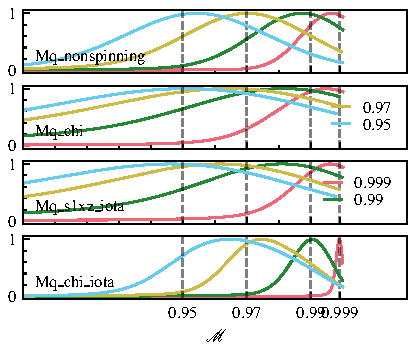
\includegraphics{metric_accuracy_hessian}
	\caption{Metric accuracy study for different manifolds.
	Each histogram shows the distribution of matches between $15000$ pairs of random points with metric match $0.95, 0.97, 0.99, 0.999$. The masses of the test points are chosen in the $M-q$ space within the rectangle ${[20, 50] M_\odot \times [1,5]}$; the other variables are chosen in the largest possible set of acceptable values.}
	\label{fig:metric_accuracy}
\end{figure}

\begin{figure*}[th!]
	\centering
	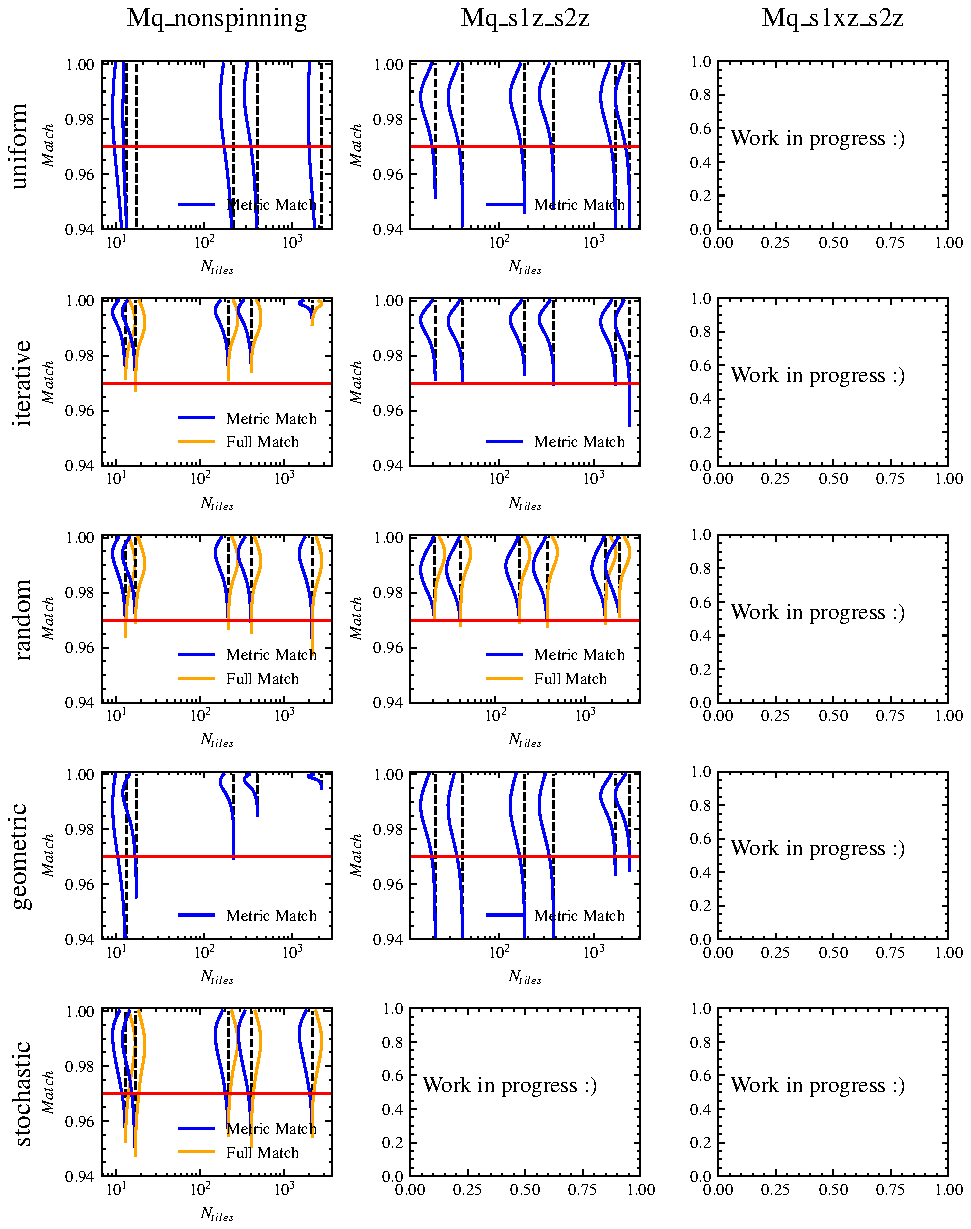
\includegraphics[width=.85\textwidth,keepaspectratio]{placing_validation}
	\caption{Results for the validation of the placing methods on $0.97$ minimum match banks. Each row refers to a different placing method whereas each column refers to a different manifold. In each plot, we report with a cross the number of tiles $N_{\text{tiles}}$ against the number of templates $N_{\text{templates}}$ of the bank.
	The diamond plot refers to the fitting factor distribution of an injection study performed on the banks. The fitting factor is computed both with the match (orange) and the metric match (blue). The histograms are normalized to arbitrary units and a red tick marks the $0.97$ match threshold. The upper limit of the histograms always corresponds to the match value of $1$ and the support extends until the 1st percentile of the distribution.
	The histograms are built with $1000$ injections for each manifold.
	}
	\label{fig:placing_validation}
\end{figure*}

As the bank generation method relies on the assumption that the metric match provides a good approximation to the match, it is crucial to have a quantitative estimation of the goodness of this assumption.

To do this, we choose 4 different manifolds of templates $\mathcal{B}$ which cover different physical quantities of interests. For each manifold, we uniformly draw $15000$ samples and we compute the metric at each point.
For each point $\theta_C$, we pick a random point at a constant metric match $\mathcal{M}_{\text{metric}}$ with respect to $\theta_C$\footnote{
This amounts to draw a point on the constant match ellipsoid centered in
$\theta_C$: $\{\theta \; | \; d_{\text{metric}}(\theta,\theta_C) \leq 1-\mathcal{M}_{\text{metric}} \}$.
}
For each pair, we compute the actual match~\eqref{eq:match} and we plot the histogram of such values. For an increasingly accurate metric approximation, we should see an increasingly narrow histogram peaked around $M_{\text{metric}}$.
We repeat the experiment for $\mathcal{M}_{\text{metric}} = 0.95, 0.97, 0.99, 0.999$.

The experiment is performed on the following manifolds:
\begin{itemize}
	\item \texttt{Mq\_nonspinning} with coordinates $M = m_1+m_2, q = m_1/m_2>1$ in the rectangle $[20, 50] M_\odot \times [1,5]$
	\item \texttt{Mq\_chi} with coordinates $M, q, \chi = s_{1z} = s_{2z}$ in the rectangle $[20, 50] M_\odot \times [1,5] \times [-0.99, 0.99]$
	\item \texttt{Mq\_s1xz\_iota} with coordinates $M, q, s_{1}, \theta_1, \iota$ in the rectangle $[20, 50] M_\odot \times [1,5] \times [0, 0.99] \times [0,\pi]  \times [0,\pi]$, where $s_1, \theta_1$ are the polar coordinates of $(s_{1x}, s_{1z})$
	\item \texttt{Mq\_chi\_iota} with coordinates $M, q, \chi, \iota$ in the rectangle $[20, 50] M_\odot \times [1,5] \times [-0.99, 0.99] \times [0,\pi]$. We employ an HM approximant
\end{itemize}

For the first two manifolds we use the approximant \texttt{IMRPhenomD} \cite{PhysRevD.93.044006, PhysRevD.93.044007}, whereas for the latter two we use \texttt{IMRPhenomPv2} \cite{PhysRevLett.113.151101} and \texttt{IMRPhenomXPHM} \cite{PhysRevD.103.104056}. The frequency range for the metric computation is always set to be $[10, 1024]Hz$.
The results are reported in fig.~\ref{fig:metric_accuracy}.

%\begin{figure}[t]
%	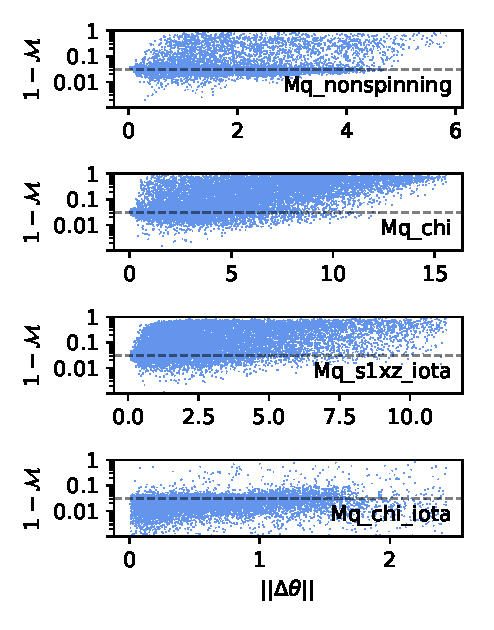
\includegraphics{metric_accuracy_hessian_distance}
%	\caption{For each pair of point with constant metric match of $0.97$ (i.e. mismatch of $0.03$, as marked by the dashed line), we report the actual mismatch as a function of coordinate distance $||\Delta\theta||$.
%	}
%	\label{fig:metric_accuracy_distance}
%\end{figure}
We first consider the first three manifolds, covered with a non-HM approximant.
By looking at the results in fig.~\ref{fig:metric_accuracy}, we observe a very large scatter in the match values between points at constant metric match: this seems to challenge the accuracy of the metric match.
However, as discussed above, the metric approximation to the match Eq.~\eqref{eq:metric_definition}, coming from a Taylor expansion, is guaranteed to be valid whenever the higher order terms of the expansion are small (e.g. at third order $H^{(3)}_{ijk}\Delta\theta_i\Delta\theta_j\Delta\theta_k$). To quantify this, one should compute the full Taylor expansion, which is expensive and out of the scope of the work.
We can limit ourselves to note that higher order terms tend to become negligible as $||\Delta\theta||$ becomes smaller.
%
%To clarify this point, in fig.~\ref{fig:metric_accuracy_distance} we plot, for each of the $15000$ pairs of points considered, the mis-match $1-\mathcal{M}$ against the coordinate distance $||\Delta\theta||$. We consider only pairs of points with constant metric distance $\mathcal{M}_{\text{metric}} = 0.97$. The trend is clear: for increasingly larger values of $||\Delta\theta||$, the higher order terms become more important, hence the accuracy of the metric approximation degrades.
%
Despite a large number of points with low accuracy, the template placing does not seem to be affected by this. Indeed, the fitting factors of a set of injections is properly estimated by the metric match, as shown in Figs.\ref{fig:placing_validation}-\ref{fig:bank_injections}.

The picture changes by inspecting the manifold \texttt{Mq\_chi\_iota}, which includes Higher Order Modes (HM).
The metric approximation consistently {\it underestimates} the actual match and provides a lower limit to the true match, yielding systematically smaller values of the match.
%This does not depend on the coordinate distance $||\Delta\theta||$ between points.
This bias is consistent with the injection study for the HM bank generated in Sec.~\ref{sec:HM_bank}, which shows a large discrepancy between metric match and true match.
The reason for such different qualitative behaviour is still unknown and requires more investigation. 


\begin{table*}[t!]
	%\centering
	\setlength\extrarowheight{1pt}
	 \begin{tabular}{l l c c c c} 
	 \hline
	 	%header
	 \multicolumn{1}{c}{\phantom{Bank name}} & \multicolumn{1}{c}{\textbf{Ranges}} & 
	 \multicolumn{2}{c}{
		\begin{tabular}{c c} \multicolumn{2}{c}{\textbf{Size}}  \\ \texttt{sbank} & \texttt{mbank} \\ \end{tabular}	 
	 } &
	  \multicolumn{2}{c}{
		\begin{tabular}{c c} \multicolumn{2}{c}{\textbf{Time}}  \\ \texttt{sbank} & \texttt{mbank} \\ \end{tabular}	 
	 }\\	 
	 %\multicolumn{1}{c}{\phantom{Bank name}} & \multicolumn{1}{c}{\textbf{Ranges}} & \multicolumn{2}{c}{\textbf{Size}} \\	 
	 %\multicolumn{1}{c}{\phantom{Bank name}} & \multicolumn{1}{c}{\phantom{Ranges}} & \multicolumn{1}{c}{\texttt{sbank}} & \multicolumn{1}{c}{\texttt{mbank}} \\
	 \hline
	 Nonspinning & \begin{tabular}{@{}l@{}} $M\in [30,50] M_\odot$ \\ $q\in [1,5]$   \\ \end{tabular}  &
	 		396 & 371 & $O(\text{hours})$ & $O(\text{seconds})$ \\
	 \cdashline{1-6}
	 Aligned spin & \begin{tabular}{@{}l@{}} $M\in [30,50]$ \\ $q\in [1,5]$ \\ $s_{1z}, s_{2z}\in [-0.99,0.99]$  \\ \end{tabular}  &
	 	3275 & 4117 & $O(\text{days})$ & $O(\text{minutes})$ \\
	 \cdashline{1-6}
	 Aligned spin low mass & \begin{tabular}{@{}l@{}} $M\in [10,30]$ \\ $q\in [1,5]$ \\ $s_{1z}, s_{2z}\in [-0.99,0.99]$  \\ \end{tabular}  &
	 	62009 & 80524 & $O(\text{months})$ &  $O(\text{hours})$\\
	 \hline
	 \end{tabular}
	 \caption{Comparison between the performance of \texttt{mbank} and  \texttt{sbank} on 3 chosen regions of the parameter space.
	 For each bank, we report the range of parameters covered by the templates, the size of the banks generated by the two methods as well as the order of magnitude of the generation time. The frequency range for all the banks is set to be $f\in [15,1024] Hz$.
	 The details of the injection studies are shown in figure~\ref{fig:sbank_comparison}.
	 The comparison are made on a machine with CPU Intel(R) Xeon(R) CPU E5-2630 installed.
	 }
 	 \label{tab:sbank_comparison}
\end{table*}

\subsection{Placing methods accuracy} \label{sec:placing_accuracy}

Here we compare the properties of different placing methods: \textit{uniform}, \textit{random} and \textit{stochastic}.
This will be helpful to understand their ranges of applicability and possible limitations in their use.

We consider 3 different manifolds:
\begin{itemize}
	\item \texttt{Mq\_chi} with coordinates $M, q, \chi $ in the rectangle $[40, 50] M_\odot \times [1,5] \times [-0.99, 0.99]$
	\item \texttt{Mq\_s1xz} with coordinates $M, q, s_{1}, \theta_1$ in the rectangle $[40, 50] M_\odot \times [1,5] \times [0, 0.99] \times [0,\pi]$
	\item \texttt{Mq\_s1xz\_s2z\_iota} with coordinates $M, q, s_{1}, \theta_1, s_{2z}, \iota$ in the rectangle $[40, 50] M_\odot \times [1,5] \times [0, 0.99] \times [0,\pi] \times [-0.99, 0.99] \times [0, \pi]$
\end{itemize}
For the first manifold we use the approximant \texttt{IMRPhenomD}, while we use \texttt{IMRPhenomPv2} for the others.
For each manifold, we generate several tilings with a different number of tiles (obtained setting a different value of \texttt{max-depth}) and we generate a bank with $0.97$ minimum match.
To compute the metric, we use the PSD for Handford measured on the first three months of the third observing run (O3), as publicly released by the LVK collaboration \cite{O3a_PSDs}.
We consider a frequency window between $10Hz$ and $1024Hz$.

We report the histogram of the fitting factors for both the match and the metric match, computed on a set of $1000$ injections.
For the stochastic placement we set the parameter $N_{max} = 200$, while for the random method we employ $10000$ livepoints.
The results are shown in fig.~\ref{fig:placing_validation}.

According to Eq.~\eqref{eq:N_templates}, the number of templates $N_{\text{templates}}$ placed by the {\it uniform} method is a measure of the volume of the space. For this reason, it is interesting to look how the number of templates placed by the {\it uniform} method depends on the number of tiles.
We note that $N_{\text{templates}}$ grows with the number of tiles until a certain upper limit. This behaviour is expected as an increasing number of tiles provides a better estimation of the overall volume of the space, until the estimation converges to the true value in the limit of large number of tiles. 

Depending on the dimensionality of the manifold, the different placing methods have different performance.
In the low dimensional manifolds \texttt{Mq\_chi} ($D=3$) and \texttt{Mq\_s1xz} ($D=4$), the {\it uniform} method has very poor performance and underestimates the number of templates. In the same two manifolds, the {\it stochastic} method performs very well and the {\it random} method gives a satisfying injection recovery, at the price of a large number of templates (3 times larger than those placed by the stochastic method).

The situation changes for the manifold \texttt{Mq\_s1xz\_s2z\_iota} ($D=6$), where the three methods show similar properties. The best performance is achieved by the {\it random} method, once again, at the cost of a large number of templates.
This is obtained thanks to the iterative control of the bank coverage, made by means of livepoints. On the other hand, since there is no control of the mutual distance between a proposal and the rest of the bank, it is very likely that some regions will be overcovered (i.e. some templates will be too close to each other).
The {\it uniform} method provides a more realistic number of templates than in the other examples. Moreover, it shows similar features as the {\it stochastic} method, both in terms of templates number and injection recovery.
In high dimensions, the control over the spacing of the templates performed by the {\it stochastic} method is not crucial anymore and provides only moderate improvement (or no improvement at all) over {\it uniform} or {\it random} methods. As discussed before, this is a well known features \cite{Messenger:2008ta, Allen:2021yuy, Allen:2022lqr} of high dimensional template banks and it makes the {\it random} (and similarly the {\it uniform}) method very appealing to cover a high dimensional region of the parameter space.

As a final remark, we note that the fitting factors computed with the metric match are widely consistent with those computed with the ``true" match. This shows the robustness of the metric approximation, despite the problems highlighted in Sec.~\ref{sec:metric_accuracy}.

%An analysis of the different methods shows that the {\it uniform} placing method has a poor performance for the low dimensional manifolds \texttt{Mq\_chi} and \texttt{Mq\_s1xz}, while still provides acceptable injection recovery for the large dimensional manifold \texttt{Mq\_s1xz\_s2z\_iota}. This was widely expcted. In low dimenensional manifolds, Eq.~\eqref{eq:N_templates} undestimates the number of templates and, since it does not check for boundaries, it provides poor coverage. This changes for high dimensional manifold, where the number of templates placed is consistent with the other methods and the coverage is satisfying, As discussed before, this is a well known features \cite{Messenger:2008ta, Allen:2021yuy, Allen:2022lqr} of high dimensional template banks and it makes the unform (and similarly the random) method very appealing to cover quickly a high dimensional region of the parameter space.

%The {\it random} method provides a very high injection recovery at the price of a very large number of templates. As shown in fig.~\ref{fig:placing_validation}, manifolds \texttt{Mq\_s1xz} and \texttt{Mq\_s1xz\_s2z\_iota} are covered with around three times more templates than those placed by the other methods.The improved over the {\it uniform} method are obtained thanks to the iterative control of the bank coverage, made by means of livepoints. On the other hand, since there is no control of the mutual distance between a proposal and the rest of the bank, it is very likely that some regions will be overcovered (i.e. some templates will be too close to each other).

%The {\it stochastic} method is able to cover the low dimensional manifold with the appropriate minimum match. Moreover, the bank size does not depend on the number of tiles. This very nice performance is expected: this placing method (with some variations) is the state of the art of bank generation and has proven to be reliable in past years. The price to pay for such nice performance is a larger bank generation time when compared with the other two methods: indeed, a lot of computational power is spent on computing mutual distances between the templates, which makes this method slower and at the same time more accurate.


\begin{figure}[t!]
	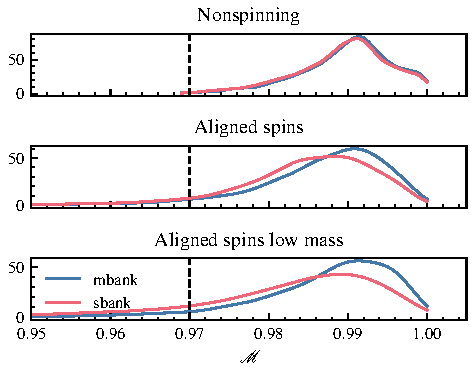
\includegraphics{sbank_comparison}
	\caption{
	Cumulative distribution of the fitting factors of the banks used to compare \texttt{mbank} and \texttt{sbank}. For each parameter space considered, we randomly draw $5000$ points (injections) from the tiling used to generate the \texttt{mbank} bank and we compute the fitting factor of these injections against the two banks. We report the distribution of fitting factor in the histograms. For visualization purposes, we plot the $0.97$ line, which corresponds to the minimum match of the banks.
	The details of the banks generated are reported in table~\ref{tab:sbank_comparison}.
	}
	\label{fig:sbank_comparison}
\end{figure}

\begin{figure}[t!]
	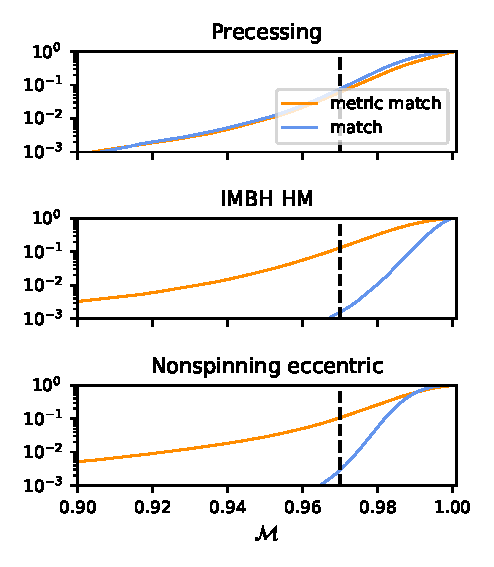
\includegraphics{bank_injections}
	\caption{
	Cumulative distribution of the fitting factors of the three case study banks. For each bank, we randomly draw $75000$ points (injections) from the tiling and we compute the fitting factor of these injections against the two banks. We report the distribution of fitting factor in the histograms both for the match and the metric match. For visualization purposes, we plot the $0.97$ line, which corresponds to the minimum match of the banks.
	The details of the banks generated are reported in table~\ref{tab:casestudy_banks}.
	%\stefano{Should we make the histogram of the cumulative distribution of the match values? Maybe it's more informative}
	}
	\label{fig:bank_injections}
\end{figure}

\subsection{Comparison with \texttt{sbank} }\label{sec:sbank_comparison}

\texttt{sbank} \cite{sbank} is a very common tool used by the LIGO Scientific, Virgo and Kagra Collaborations (LVK) to generate large template banks for analysis and, as such, it has been successfully used in the past three observing runs by several pipelines.
For this reason, it is very important to compare the performance of our code against the benchmark set by \texttt{bank}. The comparison is based on the size, speed and effectualness of the banks generated.

We generate three non-precessing template banks with both codes:
\begin{itemize}
	\item A {\it non spinning} bank
	\item An {\it aligned spins} bank
	\item An {\it aligned spins low mass} bank
\end{itemize}
The ranges of the parameter space covered by the three banks are reported in table~\ref{tab:sbank_comparison}. All the banks cover the frequency range $f\in [15,1024] Hz$ and are generated using the PSD measured during the whole second observing run (O2).
For all the three banks, templates are placed with the {\it stochastic} method, with a parameter $N_{max}=300$. In fig.~\ref{fig:sbank_comparison}, we report the result of an injection study on the three pairs of banks.

The first striking feature we observe is that \texttt{mbank} consistently places around 30\% more templates than \texttt{sbank}, in the two aligned spins banks. This means that the metric template placement tends to \textit{overcover} the space: it is a known feature (also observed in \cite{Coogan:2022qxs}) and it is inherent to the use of a metric approximation: it is the price to pay for a huge speed up in the generation.

Looking at the injections fitting factor distributions in fig.~\ref{fig:sbank_comparison}, we note the fitting factor distribution of \texttt{sbank} and \texttt{mbank} are similar in their shape, even though \texttt{sbank} shows a slightly better performance than \texttt{mbank}. This suggests that, at least in this simple non-precessing parameter space, \texttt{mbank} is able to match the state-of-the-art performance in covering.

%When considering the generation times, we see that \texttt{mbank} is {\it orders of magnitude} faster than \texttt{sbank}. This huge speed up is precisely what makes \texttt{mbank} convenient, especially to cover very large volumes: it may overcover the space but it provides a substantial speed-up, making feasible the covering of new regions of the parameter space.

%%%%%%%%%%%%%%%%%%%%%%%%%%%%%%%%%%%%%%%%%%%%%%%%%%%%%%%


\begin{table*}[t!]
	\centering
	\setlength\extrarowheight{1pt}
	 \begin{tabular}{l l l c c} 
	 \hline
	 %\multicolumn{1}{c}{\phantom{Name}} & \multicolumn{1}{c}{\textbf{Ranges}} & \multicolumn{1}{c}{\textbf{Setting}} & \multicolumn{1}{c}{\textbf{Size}} \\
	 \multicolumn{1}{c}{\phantom{Bank name}} & \multicolumn{1}{c}{\textbf{Ranges}} & \multicolumn{1}{c}{\textbf{Settings}} &  
	 \multicolumn{2}{c}{
		\begin{tabular}{c c} \multicolumn{2}{c}{\textbf{Size}}  \\ $N_{\text{templates}}$ & $N_{\text{tiles}}$ \\ \end{tabular}	 
	 } \\
	 \hline
	 Precessing & \begin{tabular}{@{}l@{}} $M\in [25,100] M_\odot$ \\ $q\in [1,5]$  \\ $s_1\in [0,0.99]$ \\$\theta_1\in [0, \pi]$ \\ $f\in [15,1024] Hz$ \\ \end{tabular}  &
	 \begin{tabular}{@{}l@{}} IMRPhenomPv2 \\ $\epsilon = 0.1$ \\ \texttt{max-depth}: 10 \\ $N_{max} = 100$\\\end{tabular}  &
	 45265 & 33774 \\
	 \cdashline{1-5}
	 IMBH HM & \begin{tabular}{@{}l@{}} $M\in [50, 600] M_\odot$ \\ $q\in [1,5]$  \\ $\chi \in [0,0.99]$ \\ $f\in [10,1024] Hz$ \\ \end{tabular}  &
	 	 \begin{tabular}{@{}l@{}} IMRPhenomXPHM \\ $\epsilon = 0.2 $ \\ \texttt{max-depth}: 8 \\ $N_{max} = 100$\\ \end{tabular}  &
	 	168010 & 33792 \\
	 \cdashline{1-5}
	 Nonspinning eccentric & \begin{tabular}{@{}l@{}} $M\in [10,75] M_\odot$ \\ $q\in [1,5]$ \\ $e \in [0,0.3]$ \\ $f\in [15,1024] Hz$ \\ \end{tabular}  &
	 	 \begin{tabular}{@{}l@{}} EccentricFD \\ $\epsilon = 0.1$ \\ \texttt{max-depth}: 9 \\ $N_{max} = 100$\\   \end{tabular}  &
	 	115748 & 4238 \\
	 \hline
	 \end{tabular}
	 \caption{Summary of three case study banks generate with \texttt{mbank}. For each bank generated, we report the variables being sampled and their ranges. We also report the approximant and the hyperparameters $\epsilon$ and \texttt{max-depth} used for the tiling generation as well as the bank size $N_{\text{templates}}$  and the number of tiles $N_{\text{tiles}}$. An injection study is performed in fig.~\ref{fig:bank_injections}. The templates distribution of the three banks is reported in fig.~\ref{fig:bank_scatter}.}
 	 \label{tab:casestudy_banks}
\end{table*}


\begin{figure*}[t]
	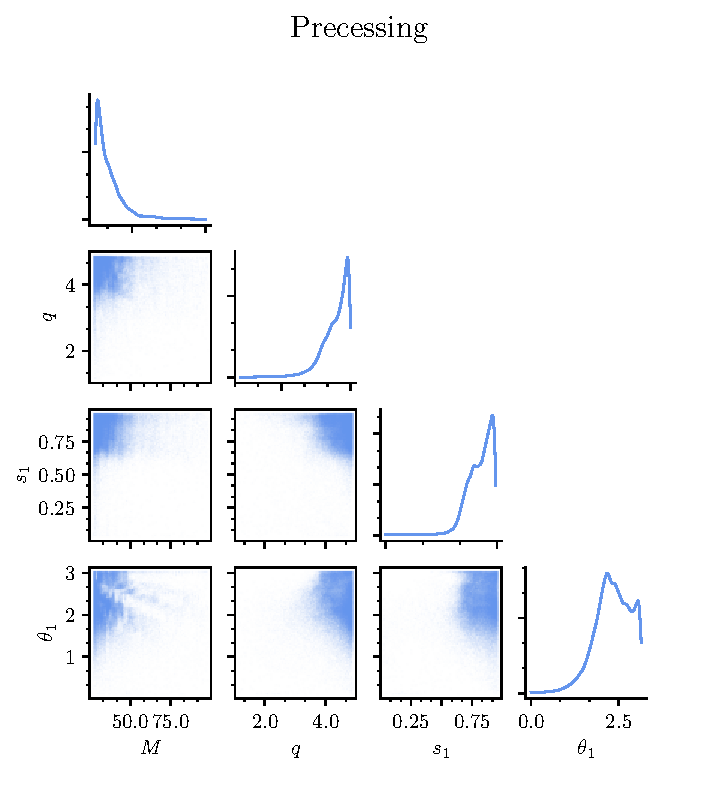
\includegraphics[scale = 0.7]{bank_scatter_Precessing}\hfill
	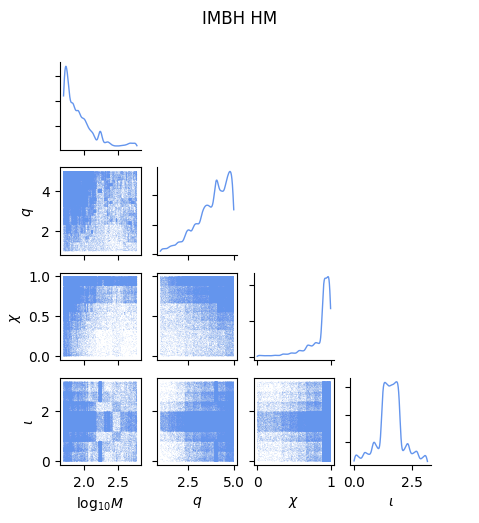
\includegraphics[scale = 0.7]{bank_scatter_IMBH_HM}\hfill
	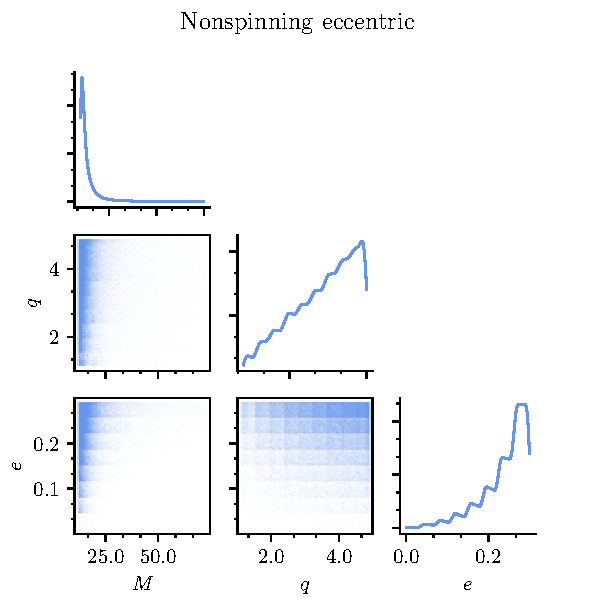
\includegraphics[scale = 0.7]{bank_scatter_Nonspinning_eccentric}
	\caption{Corner plots showing the templates for the three banks described in table~\ref{tab:casestudy_banks}. }
	\label{fig:bank_scatter}
\end{figure*}

	%%%%%%%%%%%%%%%%%%%%%%%%%%%%%%%%%
\section{Bank generation: three case studies} \label{sec:bank_generation}

To demonstrate the capabilities of our method, we use \texttt{mbank} to generate three large banks, covering interesting regions of the parameter space.
They are:
	\begin{itemize}
		\item A precessing bank
		\item An Intermediate Mass BH (IMBH) bank with Higher Order Modes
		\item A nonspinning eccentric bank
	\end{itemize}
Generating these banks with a standard approach is extremely costly and they represent the ideal situation where \texttt{mbank} is useful.

For each bank, we perform an injection study, as described in Sec.~\ref{sec:sbank_comparison}.
We generate $75000$ injections randomly drawn from the tiling: the results are reported in fig.~\ref{fig:bank_injections}. We also plot the templates of the banks in fig.~\ref{fig:bank_scatter}.
In table~\ref{tab:casestudy_banks}, we summarize the features of each bank, such as the size and the range of physical quantities that they cover.
All the banks are generated with a minimum match $MM$ requirement of $0.97$, using the {\it stochastic} placement method.
As above, we use the Hanford detector PSD measured during O3, as publicly released by the LVK collaboration \cite{O3a_PSDs}.

\subsection{A precessing bank}\label{sec:precessing_bank}
	
In our high mass {\it precessing} bank, we assign a two dimensional precessing spin to the most massive BH, by considering only the x and z components of the spin $s_1$, sampled in polar coordinates. The masses are sampled in the space (total mass - mass ratio) $M,q$.  Thus the metric is evaluated at the coordinates point $\theta = (M, q, s_1, \theta_1)$. In table~\ref{tab:sbank_comparison}, we report the ranges covered by each of this quantities. We use the approximant \texttt{IMRPhenomPv2}.

This choice of variable is based on the fact that the effect of precession can be absorbed in a single {\it effective spin parameter}, assigned to the most massive BH of a binary \cite{PhysRevD.91.024043, PhysRevD.103.083022}. Thus this physical approximation allows us to cover a large number or precessing signal using a (relatively) small number of variables.

By looking at the scatter plots of the templates fig.~\ref{fig:bank_scatter}, it is manifest the effect due to the discretization error introduced by the tiles: this causes a discontinuity in the template density. Of course, this effect is unphysical and would have been avoided by a purely stochastic placing method.
Another possible source of discontinuity can be traced back to numerical noise in the numerical gradients of the waveforms. Depending on the approximant, the gradients (hence the metric) may not behave smoothly all across the parameter space, thus explaining (partly) the hard discontinuities.

The injection recovery (fig.~\ref{fig:bank_injections}) is satisfying, with less than $10\%$ of the $75000$ injections performed having a recovery less than the target match $MM = 0.97$.
We also note that the true fitting factors and the ones approximated by the match are consistent between each other.
The bank coverage can be straightforwardly improved by setting a more stringent termination requirement $N_{max}$, which will add more templates with an improvement in injection recovery.

\subsection{An IMBH HM bank}\label{sec:HM_bank}

We generate a bank, covering the Intermediate Mass Black Hole (IMBH) region, that includes Higher Order Modes (HM). As they are more important in the strong gravity regime, they affect mostly the late inspiral and the merger part of the waveform.
For this reason, it is interesting to search HM data in the IMBH region, characterized by a total mass $M>50 M_\odot$. An IMBH signal spends only a small time ($O(ms)$) in the detector's frequency band and thus an accurate HM template is crucial for better detection.
We include in the bank the variables $\log M, q, \chi, \iota$, where $\chi=s_{1z}=s_{s2z}$ is the effective spin parameter and $\iota$ is the inclination angle.
As before in table~\ref{tab:sbank_comparison}, we report the ranges for each of this quantities. We use the modern HM approximant \texttt{IMRPhenomXPHM}.

The inclusion of HM makes the bank much larger (in other words the volume of the space is larger): for reference, a non HM bank, covering the masses and $\chi$ ranges (of course, without $\iota$) has $\sim 1000$ templates: that is a 2 orders of magnitude difference!

By looking at the injection recovery fig.~\ref{fig:bank_injections} it is striking the discrepancy between the fitting factor computed by the metric and the un-approximated one. Indeed, in the HM case the metric strongly {\it underestimates} the match, yielding an overpopulated bank. With the {\it metric} injection recovery, approximately $12\%$ of the injections have a recovery below $0.97$: this is consistent with the placing method used, which only ``knows" about metric matches. On the other hand, only $\sim 0.3\%$ are below the $0.98$ recovery factor: the bank generated is effectively a $98\%$ bank.
This effect is consistent with what observed in fig.~\ref{fig:metric_accuracy} and it is only observed whenever an HM approximant is used: as discussed above, the cause of this is unknown and requires more investigation.

\subsection{An eccentric nonspinning bank}\label{sec:eccentric_bank}

Usually the BBH searches have focused on circular orbits.
This is well theoretically motivated, as by the time of merger, any initial orbital eccentricty will be radiated away. Nevertheless is interesting to search such signals as their detection will provide invaluable information on the BBH dynamics and the BBH formation channels and stellar evolution.
The eccentricity leaves a characteristic signature on the inspiral, thus it will be more detectable on long signals. For this reason, we focus on the {\it low} mass region $M\in [10,75] M_\odot$, where the inspiral is detectable for a longer time.
To generate our eccentric bank, we use the approximant \texttt{EccentricFD} \cite{PhysRevD.93.124061} and we limit ourself to low eccentricities $e<0.3$, where the WF modelling is more reliable. Being a Post-Newtonian model, it does not include the merger and the waveform are cut in the late inspiral, as done by the code \texttt{lalsimulation} \cite{lalsuite}. Of course, this removes interesting physics and the resulting bank is expected to have a lower number of templates than what obtained using a fully eccentric approximant.

As in the case of the HM bank, the addition of eccentricity delivers a bank orders of magnitude larger than a standard non-eccentric bank.
Moreover, by looking at the fitting factor distributions, we note that, similarly to the IMBH case, the metric {\it underestimates} the match. Again, the origin of this is still under investigation.

From the scatter plot fig.~\ref{fig:bank_scatter}, we note that the discontinuities introduced by the metric are less visible. This is due to the smaller dimension of the space (3 against 4 of the previous cases), which makes easier to cover the space with a reliable tiling. Moreover, since the approximant \texttt{EccentricFD} is analytic, the metric has a smoother dependence on the parameter space, which may also help to avoid discontinuities in template density.

\section{Final remarks and future prospects} \label{sec:conclusion}

We present a novel method to generate template banks to cover a high dimensional manifold of (possibly) precessing/HM/eccentric BBH signals.
We rely on the metric approximation to the match Eq.~\eqref{eq:metric_definition} to compute distances between points and we set up an algorithm to create a tiling of the manifold. Given a tiling, we are able to implement several strategies to place templates to cover the space with a given minimum match target.
The code implementing our method is publicly available as a package \texttt{mbank} and it comes with a number of tools to make the bank generation and validation easy.

To validate our method, we compared the output of our code to the one of the state-of-the-art \texttt{sbank}: we find that mbank is able to faithfully cover the space, although with a larger number of templates when compared with \texttt{sbank}.
To demonstrate the capabilities of our code, we generated three banks covering some interesting and up to now unexplored regions of the parameter space. We found the \texttt{mbank} is able to provide a faithfully coverage.
The banks generated are ready to be employed in real GW searches.

\texttt{mbank} is order of magnitude faster than the non-metric state-of-the-art bank generation codes. This makes our code particularly suitable for a large dimensional parameter space and makes feasible the generation of banks for which the template placing was hitherto unfeasible, due to computational limitations.
This was possible thanks to two innovative features:
\begin{itemize}
	\item The metric is used consistently everywhere throughout the package
	\item The tiling provides a fast and efficient interface to the metric, making tractable hard problems such as volume estimation and template sampling
\end{itemize}

Our work can be improved and extended in several directions:
\begin{itemize}
	\item {\it Improving the metric computation} As discussed in Sec.~\ref{sec:metric_accuracy}, the metric accuracy may not be optimal, especially for large coordinate distance $||\Delta\theta||$. While this has proven not to affect negatively the template placing, it would still be desiderable to have a better estimation of the match. Future developments can work in this direction by solving the problem in Eq.~\eqref{eq:metric_optmization} or even departing from the bilinear approximation\footnote{
Although this latter strategy may sound tempting, it would cease to provide a meaningful estimation of volume, which may be problematic for template placement.} of Eq.~\eqref{eq:metric_definition}.
	
	\item {\it Investigate the performance for HM}. We observed in Sec.~\ref{sec:HM_bank} that the metric placement overcovers the space, due to the fact that the metric underestimates the match. This is puzzling and it requires more investigation.
	
	\item {\it Interpolate between different tiles} Due to the discrete nature of the tiles, a bank can show large discontinuities on the template densities. While this may not be a problem for matched filter searches, avoiding this could improve the bank performance by reducing the bank size without affecting the its effectualness. To create a smooth dependence of the metric on the parameter space, we could set up an interpolation scheme, based on the tiling.
	
	\item {\it Post process the bank} Regardless of the placing method, the templates in a bank may not be placed optimally, creating over(under)dense regions. This is especially true for the {\it random} placing method. It may be good to add a post-processing step to move or remove some templates: this would rely on a large injection set to trim the bank. The overall result can be a smaller bank with better covering properties \cite{Indik:2017vqq}.
\end{itemize}

As a final remark, we emphasize that our work enables the GW community to run searches on novel regions of the BBH signals parameter space. By cutting the bank generation and validation time by orders of magnitude, the computational cost of searching new regions of the parameter space will be dominated by the actual cost of the analysis rather than the cost of prior steps.
This will allow for optimal resource allocation to search for signature of precession, eccentricity and/or HMs, hopefully leading to new exciting physics.

	%%%%%%%%%%%%%%%%%%%%%%%%%%%%%%%%% ACKNOWLEDGMENTS
        \begin{acknowledgments}
		S.S. and S.C. are supported by the research program of the Netherlands Organisation for Scientific Research (NWO).
		The authors are grateful for computational resources provided by the LIGO Laboratory and supported by the National Science Foundation Grants No. PHY-0757058 and No. PHY-0823459. This material is based upon work supported by NSF’s LIGO Laboratory which is a major facility fully funded by the National Science Foundation.
        \end{acknowledgments}

	%%%%%%%%%%%%%%%%%%%%%%%%%%%%%%%%% APPENDIX
\newpage
\appendix
\section{Details of the metric computation}\label{app:metric}

In this appendix we report the details of the derivation of the expression~\eqref{eq:metric_expression}, as well as the computation of the Hessian $H$ of the overlap Eq.~\eqref{eq:overlap} in terms of the gradients of the waveform $h(\theta)$. 
In what follows, we define $\rescalar{h_1}{h_2}$ and $\imscalar{h_1}{h_2}$ to be respectively the real and imaginary part of $\scalar{h_1}{h_2}$.

We begin by expanding the quantity $\mathcal{M}(\theta,\theta +\Delta\theta)$ for $\Delta\theta$ around $0$. Since the $\mathcal{M}(\theta,\theta +\Delta\theta)$ has a maximum for $\Delta\theta = 0$, the leading term is quadratic in $\Delta\theta$.
We obtain:
\begin{align} \label{eq:metric_derivation}
	&\mathcal{M}(\theta,\theta +\Delta\theta) = \max_{\Delta t} \mathcal{O}(\theta, \theta + \Delta\theta, \Delta t) \nonumber\\
	& =	\max_{\Delta t} \left\{ 1+ \frac{1}{2}\left[ \partial_{ij}\mathcal{O} \Delta\theta_i \Delta\theta_j + 2  \partial_{it}\mathcal{O} \Delta\theta_i \Delta t + \partial_{tt}\mathcal{O} (\Delta t)^2 \right] \right\}  \nonumber \\
	&= 1 + \frac{1}{2}\left[ \partial_{ij}\mathcal{O} - \frac{\partial_{it}\mathcal{O} \partial_{jt}\mathcal{O}}{\partial_{tt}\mathcal{O}}\right] \Delta\theta_i \Delta\theta_j
\end{align}
where all the derivatives are evaluated at ${\Delta\theta = \Delta t = 0}$ and the explicit time maximization yields
${\Delta t = -\frac{\partial_{it}\mathcal{O} \Delta\theta_i}{\partial_{tt}\mathcal{O}}}$.

From the above Eq.~\eqref{eq:metric_derivation}, we can read the expression for the metric in Eq.~\eqref{eq:metric_expression} recognizing in the derivatives $\partial\partial\mathcal{O}|_{\Delta\theta, \Delta t = 0}$ the components of the Hessian matrix $H$ of the overlap.

We now compute the Hessian of the overlap as a function of the gradients of the {\it normalized} waveforms.
We have\footnote{
A constant factor in front of the frequency in the fourier transform does not affect the result. For this reason, we dropped the constant $2\pi$ in the exponential.}:
\begin{align}
	\partial_i \mathcal{O} &= \frac{1}{\mathcal{O}} \left[ \rescalar{\hat{h}}{\hat{h}e^{ift}}\rescalar{\hat{h}}{\partial_i\hat{h}e^{ift}} + \imscalar{\hat{h}}{\hat{h}e^{ift}}\imscalar{\hat{h}}{\partial_i\hat{h}e^{ift}} \right]\\
	\partial_t \mathcal{O} &= \frac{1}{\mathcal{O}} \left[ \rescalar{\hat{h}}{\hat{h}e^{ift}}\rescalar{\hat{h}}{\hat{h}if e^{ift}} + \imscalar{\hat{h}}{\hat{h}e^{ift}}\imscalar{\hat{h}}{\hat{h}if e^{ift}} \right]
\end{align}
Differentiating another time, after some rearrangements, we get:
\begin{align}
H_{tt} &= \frac{\partial^2 \mathcal{O}}{\partial t \partial t } \left|_{\Delta\theta, t = 0} \right.
								= \rescalar{\hat{h}}{\hat{h}f}^2 - \rescalar{\hat{h}}{\hat{h}f^2} \label{eq:H_tt}\\
H_{ti} &= \frac{\partial^2 \mathcal{O}}{\partial \Delta \theta_i \partial t } \left|_{\Delta\theta, t = 0} \right.
								= - \imscalar{\hat{h}}{\partial_i \hat{h}f} + \imscalar{\hat{h}}{\partial_i\hat{h}} \rescalar{\hat{h}}{\hat{h}f} \label{eq:H_ti}\\
H_{ij} &= \frac{\partial^2 \mathcal{O}}{\partial \Delta \theta_i \partial \Delta \theta_j }\left|_{\Delta\theta, t = 0} \right.
								= \rescalar{\hat{h}}{\partial_i\partial_j\hat{h}} +\imscalar{\hat{h}}{\partial_i\hat{h}} \imscalar{\hat{h}}{\partial_j\hat{h}} \label{eq:H_ij}
\end{align}

To move further, we express the normalized waveform derivatives in terms of the non normalized ones. We get:
\begin{align*}
	\bullet&\quad \partial_i \scalar{h}{h} = \scalar{\partial_i h}{h}+ \scalar{h}{\partial_i h} = 2 \rescalar{h}{\partial_i h} \\
	\bullet&\quad \partial_i \hat{h} =\frac{1}{\rescalar{h}{h}^{3/2}} \left[ \rescalar{h}{h}\partial_i h -  \rescalar{h}{\partial_i h} h \right]	\\
	\bullet &\quad \partial_i \partial_j \hat{h} = \frac{1}{\rescalar{h}{h}^{1/2}} \partial_{ij}h 	+3 \frac{1}{\rescalar{h}{h}^{5/2}} \rescalar{h}{\partial_i h}\rescalar{h}{\partial_j h}h \\
	&- \frac{1}{\rescalar{h}{h}^{3/2}} \left[\rescalar{h}{ \partial_{ij} h} h + \rescalar{\partial_i h}{\partial_j h}  h
		+2\rescalar{h}{\partial_{(i} h} \partial_{j)} h \right]
\end{align*}
where $A_{(ij)} = \frac{1}{2}(A_{ij}+A_{ji})$ denotes symmetrization.

Plugging this into the equations~\eqref{eq:H_tt}-\eqref{eq:H_ij}, we get:
\begin{align}
	H_{tt} &= \frac{1}{\rescalar{h}{h}^{2}} \rescalar{{h}}{{h}f}^2 - \frac{1}{\rescalar{h}{h}} \imscalar{h}{{h} f^2 } \label{eq:H_tt_grad} \\
	H_{ti} &= \frac{1}{\rescalar{h}{h}^{2}} \Big\{ \imscalar{h}{\partial_i {h}} \rescalar{{h}}{{h}f} +\rescalar{h}{\partial_i {h}} \imscalar{h}{hf} \Big\} \nonumber \\
	&- \frac{1}{\rescalar{h}{h}} \imscalar{h}{\partial_i{h} f } \label{eq:H_ti_grad} \\
	H_{ij} &=  \frac{1}{\rescalar{h}{h}^{2}} \Big\{ \rescalar{h}{\partial_i {h}} \rescalar{{h}}{\partial_j {h}} +\imscalar{h}{\partial_i {h}} \imscalar{h}{\partial_j {h}} \Big\} \nonumber \\
	&- \frac{1}{\rescalar{h}{h}} \rescalar{\partial_i h}{\partial_j {h}} \label{eq:H_ij_grad} 
\end{align}

Such expressions, togheter with Eq.~\eqref{eq:metric_expression} fully specify the metric computation.
The gradients $\partial_i h$ of the waveform can be computed with an accurate finite difference scheme.

%\begin{equation*}
%	\mathcal{M}(\theta_1,\theta_2) =  \max_{t} \left\lvert \int\limits_{f_\text{min}}^{f_\text{max}} \d{f} \frac{\tilde{\hat{h}}^*(f;\theta_1)\tilde{\hat{h}}(f;\theta_2) e^{i2\pi ft}}{S_n(f)} \right\rvert^2
%\end{equation*}


%\begin{equation}
%	\mathcal{M}(h_1,h_2) =  1- \frac{\rescalar{h_1}{h_2}}{\sqrt{\rescalar{h_1}{h_1}\rescalar{h_2}{h_2}}}
%\end{equation}

%\begin{equation}
%	\rescalar{h_1}{h_2} = \Re \int \text{d}f \; \frac{\tilde{{h}}^*_1 \tilde{{h}}_2}{S_n}
%\end{equation}

	%%%%%%%%%%%%%%%%%%%%%%%%%%%%%%%%% BIBLIOGRAPHY
	\bibliography{biblio.bib}
	\bibliographystyle{ieeetr}

\end{document}



